\chapter{Sieci neuronowe}
\label{cha:sztuczne_sieci_neuronowe}

Rozdział ten zawiera informacje na temat historii rozwoju sieci neuronowych, ich architektury, zasady działania oraz algorytmów uczenia.

\section{Początki sztucznych sieci neuronowych}
Początki prac nad poznaniem procesów zachodzących w ludzkim mózgu datuje się na rok 1943. W pracy McCulloch'a oraz Pitts'a przedstawiono matematyczny model neuronu, który zapoczątkował badania związane z tym tematem. W 1949 roku Donald Hebb odkrył, iż informacje przechowywane w sieci neuronowej są reprezentowane jako wartości wag pomiędzy poszczególnymi neuronami. Na podstawie tych informacji zaproponował pierwszy algorytm uczenia sieci neuronowej, który został nazwany regułą Hebba. Już wtedy odkryto, iż bardzo dużą zaletą sieci jest równoległy sposób przetwarzania informacji oraz metodologia uczenia, która zastępuje tradycyjny proces programowania. Pierwszym przykładem realizacji sztucznej sieci neuronowej jest Perceptron. Został on zbudowany w 1957 roku przez Franka Rosenblatta i Charlesa Wightmana. Sieć ta została nauczona rozpoznawania znaków alfanumerycznych. Niestety projekt ten nie okazał się w pełni sukcesem, ponieważ sieć była wrażliwa na zmianę wielkości podawanych znaków oraz nie radziła sobie z bardziej skomplikowanymi. Dzieło to wzbudziło zainteresowanie na całym świecie, spowodowało popularności sieci neuronowych wśród naukowców. Powstało wiele ciekawych prac, które wpływały na rozwój tej dziedziny. Badania te zostały spowolnione przez opublikowanie w 1969 roku książki Minskiego i Paperta noszącej tytuł Perceptrons. Dowiodła ona, że jednowarstwowe sieci mają bardzo ograniczone możliwości. 
Dopiero od połowy lat 80-tych, zagadnieniem tym oprócz naukowców zaczęły się interesować firmy komercyjne. Było to spowodowane dwoma głównymi czynnikami: wydaniem książki w 1988 roku przez Jamesa Andresona oraz rozwojem technologii układów mogących modelować coraz bardziej złożone sztuczne sieci neuronowe. Dynamiczny rozwój tej dziedziny trwa do dnia dzisiejszego.

\section{Zastosowanie sieci neuronowych}
Rozwój nauki poświęconej sztucznym siecią neuronowym oraz znaczny postęp techniki umożliwia stosowanie sieci neuronowych w prawie każdej dziedzinie naszego życia. Do najważniejszych z nich można zaliczyć:

\begin{itemize}
	\item prognozy giełdowe,
	\item analizę badań medycznych,
	\item sterowanie systemem zasilania oraz chłodzenia serwerowni,
	\item optymalizację działalności handlowej,
	\item kryminalistykę,
	\item sterowanie procesów przemysłowych,
	\item przemysł lotniczy.
\end{itemize}

Ze względu na wszechstronność zastosowania sieci neuronowych oraz ich odpowiedników, służących do rozwiązywania bardziej złożonych zagadnień głębokich sieci neuronowych (ang. Deep Neural Network), stosuje się ich podział oparty na możliwościach, dedykowanych rodzinach problemu, do których zostały przystosowane zamiast dziedzin nauki do jakich są wykorzystywane.
W swojej książce prof. Ryszard Tadeusiewicz opisuje główne zastosowania sieci neuronowych \cite{tade93}:

\begin{itemize}
	\item Predykcji - ich głównym zadaniem jest przewidywanie określonych sytuacji na podstawie danych wejściowych. Zagadnienie to jest wykorzystywane do prognozy giełdowej, prognozy ekonomicznego rozwoju, prognozy rynkowej, oceny zdolności kredytowej oraz wiele innych. Wprowadzanie sieci neuronowych w takich przypadkach pozwala na przewidywanie poszczególnych wyników bez głębszego rozumienia problemu. Bardzo ważną zaletą jest brak potrzeby określania dokładnych hipotez świadczących o powiązaniu wejścia z wyjściem. Podczas procesu nauczania sieć sama dostosowuje się do zagadnienia na podstawie danych uczących. Często skutkuje to większą efektywnością w rozwiązywaniu problemów takich jak prognozy giełdowe w stosunku do tradycyjnych aplikacji. Powodem tego zjawiska jest to, iż aplikacje do gry na giełdzie bazują na wprowadzonych przez człowieka zależnościach, natomiast sieci neuronowe same dobierają sobie kryterium, według którego reagują na poszczególne wejścia.
	\item Klasyfikacji i rozpoznawania przedmiotów - zagadnienie to jest bardzo często rozwiązywane przy sztucznych sieci neuronowych. Wykorzystywane są one również w ekonomii, gdzie na podstawie wcześniej określonych etapów przyporządkuje jedne z nich do przedsiębiorstwa na podstawie wejść sieci świadczących o jego stanie. Podczas uczenia sieci wychwytuje ona charakterystyczne cechy poszczególnego wejścia, a następnie przypisuje im konkretne wyjście. Rozwiązywanie tego typu problemów za pomocą sztucznych sieci neuronowych okazuje się bardzo wygodne, ponieważ w przypadku zmiany zagadnienia wymagane jest jedynie powtórzenie procesu nauki bez ingerencji w implementację. Jest to zdecydowanie bardzo duża zaleta w stosunku do tradycyjnych aplikacji, ponieważ nie są one uniwersalne, co powoduje ogromne koszty w przypadku wszelakich modyfikacji. Często kosz poprawek jest zbliżony do kosztów tworzenia nowej aplikacji.
	\item Kojarzenia danych - bardzo często rozwiązaniem wielu problemu jest szybkie kojarzenie różnych faktów. W porównaniu do tradycyjnych systemów sieci neuronowe, dzięki zdolności uczenia oraz adaptacji, pozwalają na kojarzenie różnorodnych danych.  Skutkuje to uzyskaniem przejrzystych informacji na wyjściu sieci bez potrzeby analizy szczegółowych, nadmiarowych danych, z których wyciągnięcie wniosków wymaga żmudnej i długotrwałej analizy. 
	\item Analizy danych - zagadnienie to opiera się na wykryciu związków przyczynowo skutkowych w zbiorze wejściowym. Jest to bardzo istotny problem ze względu na częste fałszywe wnioski wyciągane przez ludzi. Sztuczne sieci neuronowe pozwalają na rzeczywiste wykrycie przyczyny sukcesu jak i niepowodzenia poszczególnych operacji. W oparciu o taki mechanizm, na podstawie przeszłości podejmowanie decyzji staje się zdecydowanie łatwiejsze, jak i również minimalizuje ryzyko popełnienia wcześniejszych błędów.
	\item Filtracji sygnałów - technika ta jest głównie wykorzystywana w telekomunikacji oraz automatycznej diagnostyce medycznej. Odgrywa ona znaczącą rolę dla rozwoju tych dziedzin. Całe zagadnienie opiera się na usuwaniu zakłóceń pochodzących z różnych źródeł. Są one wykorzystywane do wstępnej obróbki danych, z których eliminowane są nie tylko zakłócenia o charakterze losowym jak również celowe przekłamania. Dodatkowo tradycyjne metody nie mają możliwości uzupełniania niekompletnych danych, co w przypadku sztucznych sieci neuronowych odbywa się ze szczególną łatwością.
	\item Optymalizacji - jest to prawdopodobnie jedno z najważniejszych zagadnień dla każdej dziedziny nauk technicznych. Problemy te są rozwiązywane przez wykorzystywanie tzw. sieci Hopfielda, która rozwiązuje zagadnienia poszukiwania optymalnych decyzji. Sieci te są stosowane do rozwiązywania zagadnień optymalizacji kombinatorycznej, które są znane z ogromnej złożoności obliczeniowej - niektóre z nich są problemami NP-zupełnymi. Ich największym atutem jest czas, w którym znajdują rozwiązanie. Jest on nieporównywalnie mniejszy dzięki współbieżności obliczeniowej. 
\end{itemize}

Warto zaznaczyć, iż również w przypadku sterowania na bardzo dużą skalę wprowadza się algorytmy oparte na sztucznych sieciach neuronowych. Zagadnienie to jest głównym tematem niniejszej pracy, stąd zastosowanie sieci neuronowej do tych zagadnień zostało opisane w późniejszych rozdziałach.

\section{Sztuczne sieci neuronowe}
Ze względu na sposób działania, który przypomina działanie ludzkiego mózgu, sztuczne sieci neuronowe często traktowane są jako początek sztucznej inteligencji. Korzystanie z sieci neuronowych wymaga przejścia przez dwa podstawowe etapy. Pierwszy z nich określany jest jako uczenie sieci, a drugi jako testowanie, które jest używane do oceny poprawności działania sieci po jej wytrenowaniu. Istnieją różne algorytmy uczenia sieci neuronowej, najpopularniejszy z nich nazywany jest perceptronem wielowarstwowym (ang. multilayer perceptron). Polega on na propagacji danych w przód, a następnie przy użyciu algorytmu wstecznej propagacji, modyfikacji odpowiednich wag neuronów. Sztuczne sieci neuronowe są uznawane jako skuteczna metoda do rozpoznawania wzorców. W ich skład wchodzą połączenia między neuronami jak również same neurony, które równolegle przetwarzają dane wejściowe. Podejście to zostało zaczerpnięte z biologicznego systemu nerwowego.

\section{Biologiczne neurony}

Ludzki mózg składa się z milionów neuronów, które są połączone między sobą przez prawie 10 miliardów synaps. Architektura ta pozwala na równoległe przetwarzanie informacji. Ogólny schemat biologicznego neuronu został przedstawiony na rysunku \ref{fig:bio_neuron}.

\begin{figure}[!htbp]
\centering
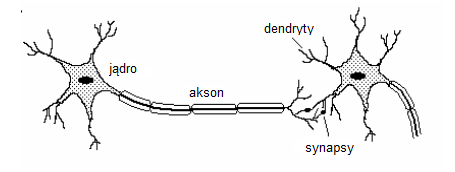
\includegraphics[width=1\linewidth]{./include/bio_neuron}
\caption{Biologiczny neuron.}
\label{fig:bio_neuron}
\end{figure}

Podstawową funkcją neuronu jest transportowanie przetworzonej informacji w postaci impulsu nerwowego, który jest reprezentowany przez krótkotrwałą zmianę potencjału. Jest on przewodzony od aksonu do synapsy, która znajduje się na jego zakończeniach. 

\section{Sztuczny neuron}
Sposób działania sztucznego neuronu jest ściśle oparty na działaniu biologicznego neuronu. Posiada on wiele wejść oraz jedno wyjście. Dla lepszego zrozumienia funkcjonowania takiego neuronu wskażmy jego różnice w stosunku do biologicznego.
Współczesne komputery posiadają bardzo dużą moc obliczeniową skupiającą się w pojedynczych procesorach taktowanych wysoką częstotliwością. W przeciwieństwie do nich ludzki mózg posiada miliardy neuronów, które przetwarzają dane wolniej niż współczesne procesory. Informacje przenoszone przez bodźce w ludzkim mózgu są reprezentowane przez logikę binarną o określonym progu aktywacji. W przypadku sztucznych neuronów funkcjonalność ta jest realizowana przez funkcje aktywacji, które na podstawie dobranego progu przypisują wartość logiczną zbliżoną do "1" dla wartości powyżej progu oraz "0" dla pozostałych. W sztucznych sieciach neuronowych po wykonaniu obliczeń w konkretnym neuronie jego wartość wyjściowa przekazywana jest wzdłuż łańcucha sieci do kolejnych neuronów. 
W celu lepszego zobrazowania działania sztucznych neuronów często są one porównywane do przekaźników. Synapsy występujące w ludzkim mózgu są odpowiednikami wag dla poszczególnych wejść neuronów.

\begin{figure}[!htbp]
\centering
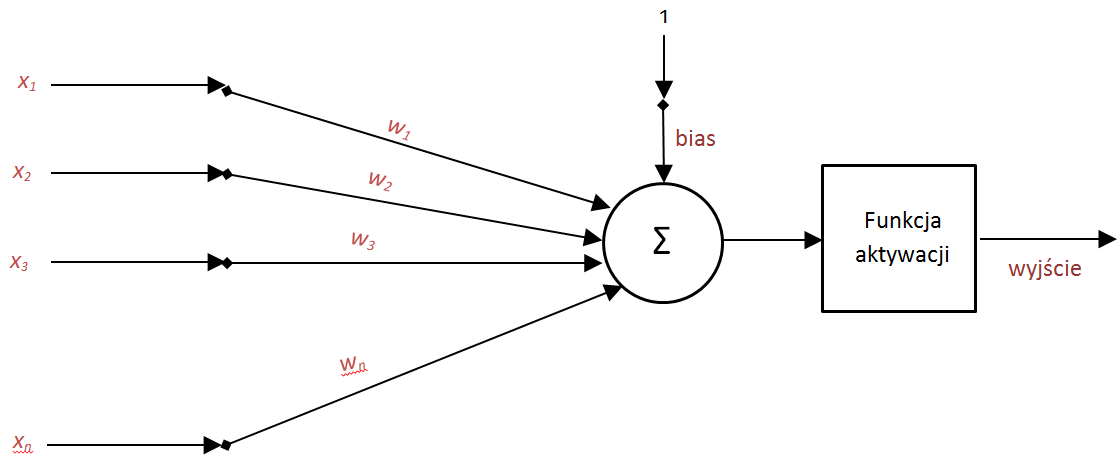
\includegraphics[width=1\linewidth]{./include/perceptron}
\caption{Sztuczny neuron.}
\label{fig:perceptron}
\end{figure}

Jak pokazano na rysunku \ref{fig:perceptron} wartości na każdym z wejść są przemnażane przez odpowiadające temu wejściu wagi. Jedno wejście posiada statyczną wartość 1. Zabieg ten umożliwia sieci neuronowej lepiej przystosowywać się do wzorców. Neuron odpowiada za sumowanie wszystkich wartości. Następnie po obliczeniu sumy ilorazów wartości sygnałów wejściowych z poszczególnymi wagami, podawana jest ona na wejście funkcji aktywacji, której wyjście jest jednoznaczne z końcową wartością uzyskaną po przetworzeniu danego wektora wartości wejściowych. 

\section{Nauka sieci}

Nawet przy dotychczasowych osiągnięciach techniki nie możliwe jest w pełni zamodelowanie pracy ludzkiego mózgu. Nie mniej jednak sztuczne sieci neuronowe pozwalają na rozwiązywanie wiele skomplikowanych zagadnień takich jak rozpoznawanie wszelkiego rodzaju wzorców oraz wiele innych. Bardzo ciekawą własnością sieci neuronowych jest to, iż nawet przy tej samej architekturze po ówczesnym przygotowaniu są w stanie one rozwiązywać całkowicie różne zagadnienia. Takie przystosowanie określane jest jako nauka sieci (ang. learning). Proces ten można porównać do okresu rozwoju noworodka, który na podstawie zdobytych doświadczeń zdobywa nowe umiejętności.
Naukę dzieli się głównie na dwie podstawowe kategorie:
\begin{itemize}
	\item nauczanie z nauczycielem (nadzorowane) (ang. supervised learning) –  podejście to wymaga nadzoru, w większości jest to zbiór oczekiwanych wartości odpowiedzi dla konkretnych wejść. Dokonuje się w nim próby przewidzenia wyników dla znanych danych wejściowych. Najbardziej znanym algorytmem w tej kategorii jest wsteczna propagacja błędów (ang. backpropagation). Polega ona na uczeniu sieci bazując na błędach. Początkowo wagi połączeń między neuronami są wybierane w sposób losowy, następnie na wejście sieci podawany jest wektor wejść ze znanymi poszczególnymi wartościami, znana  jest również wartość oczekiwana dla wyjścia. Jest ona porównywana z aktualnym wyjściem sieci, a następnie na podstawie wielkości błędu obliczana jest wartość korekcji poszczególnych wag każdego z połączeń, tak aby błąd ten został zminimalizowany. Największą wadą algorytmów tego typu jest znajomość dokładnej postaci wektora wyjściowego, która jest ciężka do spełnienia.
	\item nauczanie bez nauczyciela (nienadzorowane) (ang. unsupervised learning) - podejście to zyskało popularność ze względu na brak konieczności znajomość oczekiwanego wektora danych wyjściowych podczas uczenia sieci. W tym przypadku wyjście sieci nie jest weryfikowane. Do najbardziej znanych algorytmów reprezentujących to podejście zaliczamy sieci Kohonena - samoograniczające się odwzorowania (ang. self-organizing map). Podczas podawania kolejnych danych uczących, to na sieci spoczywa odpowiedzialność za wytworzenie odpowiednich wzorców w zależności od danych wejściowych.
\end{itemize}

Istnieje możliwość wykorzystania obydwu metod uczenia odpowiednio ze sobą złączonych, które są stosowane oraz dają najlepsze rezultaty dla bardzo złożonych problemów.
 
\section{Funkcja aktywacji}
W sieciach neuronowych funkcja aktywacji odpowiedzialna jest za przekształcenie sumy powstałej przez dodanie iloczynów poszczególnych wag z odpowiadającymi im sygnałami wejściowymi. Wyróżnia się trzy główne typy takich funkcji: progowa, liniowa, sigmoidalna. 

\subsection{Progowa funkcja aktywacji}
Progowa funkcja aktywacji została przedstawiona przez McCullon'a oraz Pits'a w 1943 roku. Prosta funkcja tego typu może być określona wzorem:


$$ 
f(x) = \left\{ \begin{array}{ll}
+1 & \textrm{gdy $x>0$}\\
-1 & \textrm{gdy $x \le 0$}\\
\end{array} \right.
$$

Funkcja ogranicza się do przypisania zadanej wartości dla wejścia powyżej progu aktywacji. W pozostałych przypadkach neuron otrzymuje stan świadczący o braku jego aktywności. Na rysunku \ref{fig:step} przedstawiono przykładowy wykres funkcji progowej.

\begin{figure}[!htbp]
\centering
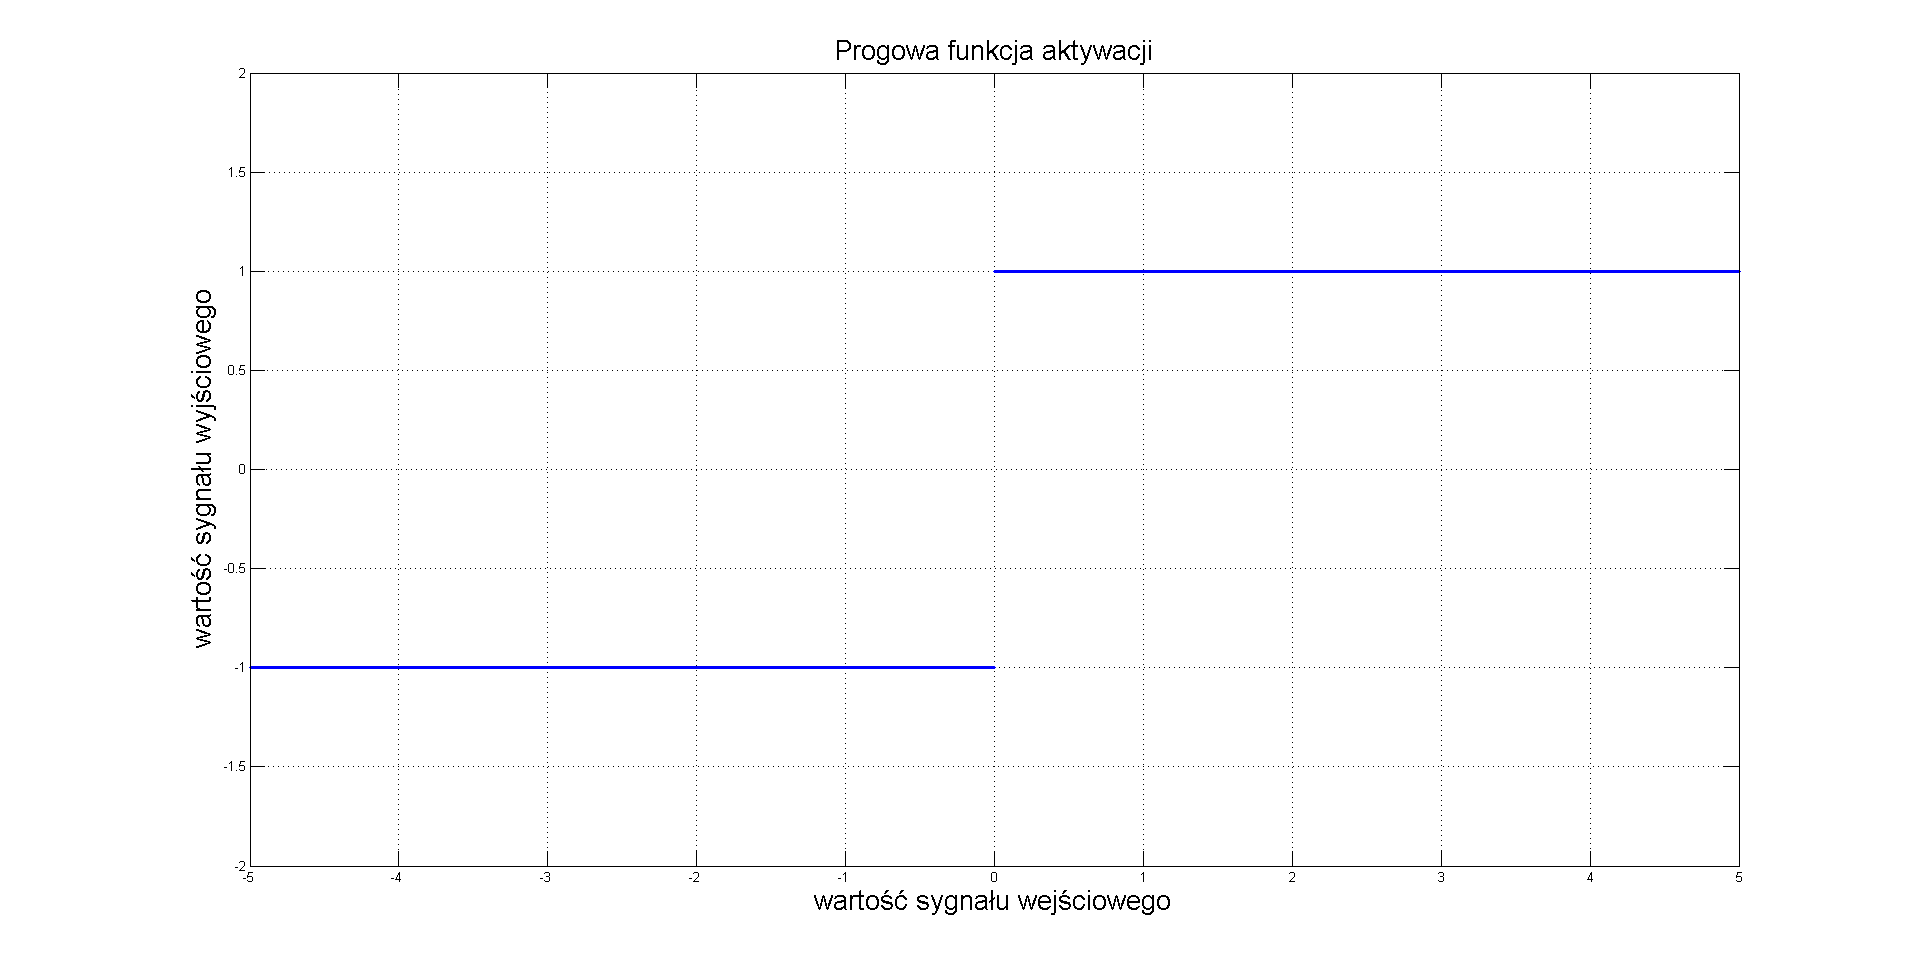
\includegraphics[width=1\linewidth]{./include/step}
\caption{Przykładowa funkcja progowa.}
\label{fig:step}
\end{figure}


\subsection{Liniowa funkcja aktywacji}
Funkcja liniowa odpowiada za liniowe przekazanie wartości wejściowej na wyjściową po przemnożeniu jej przez odpowiedni współczynnik. Dana jest ona wzorem:

$$ 
f(x) = a*x
$$

Na rysunku \ref{fig:lin} przedstawiono przykładową funkcję liniową.
\begin{figure}[!htbp]
\centering
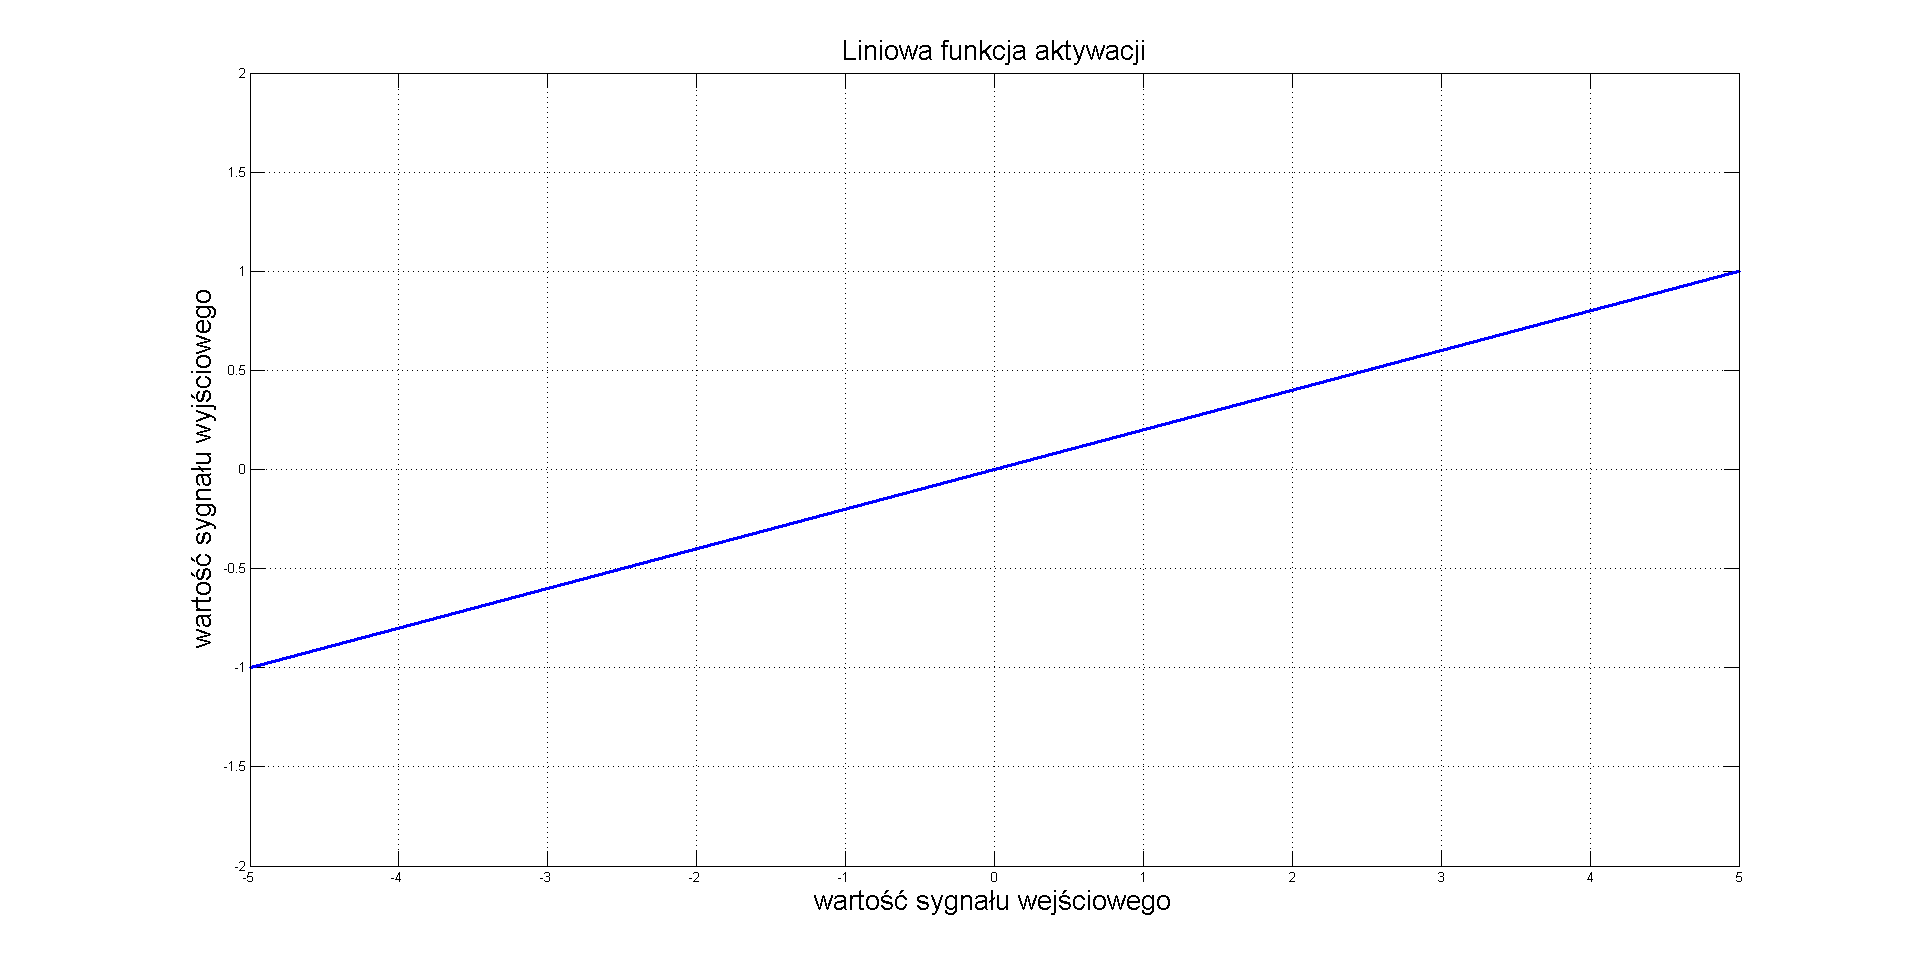
\includegraphics[width=1\linewidth]{./include/lin}
\caption{Przykładowa funkcja liniowa.}
\label{fig:lin}
\end{figure}

\subsection{Sigmoidalna funkcja aktywacji}
Funkcja sigmoidalna jest najczęściej używana w sztucznych sieciach neuronowych ze względu na jej różniczkowalność oraz zachowanie zgodne z głównymi właściwościami sieci neuronowych. Sigmoidalna funkcja unipolarna charakteryzuje się nieliniowym narastaniem w zakresie od 0 do 1. Opisana jest wzorem:

$$ 
f(x) = \frac{1}{1 + e^{-x}}
$$

\begin{figure}[!htbp]
\centering
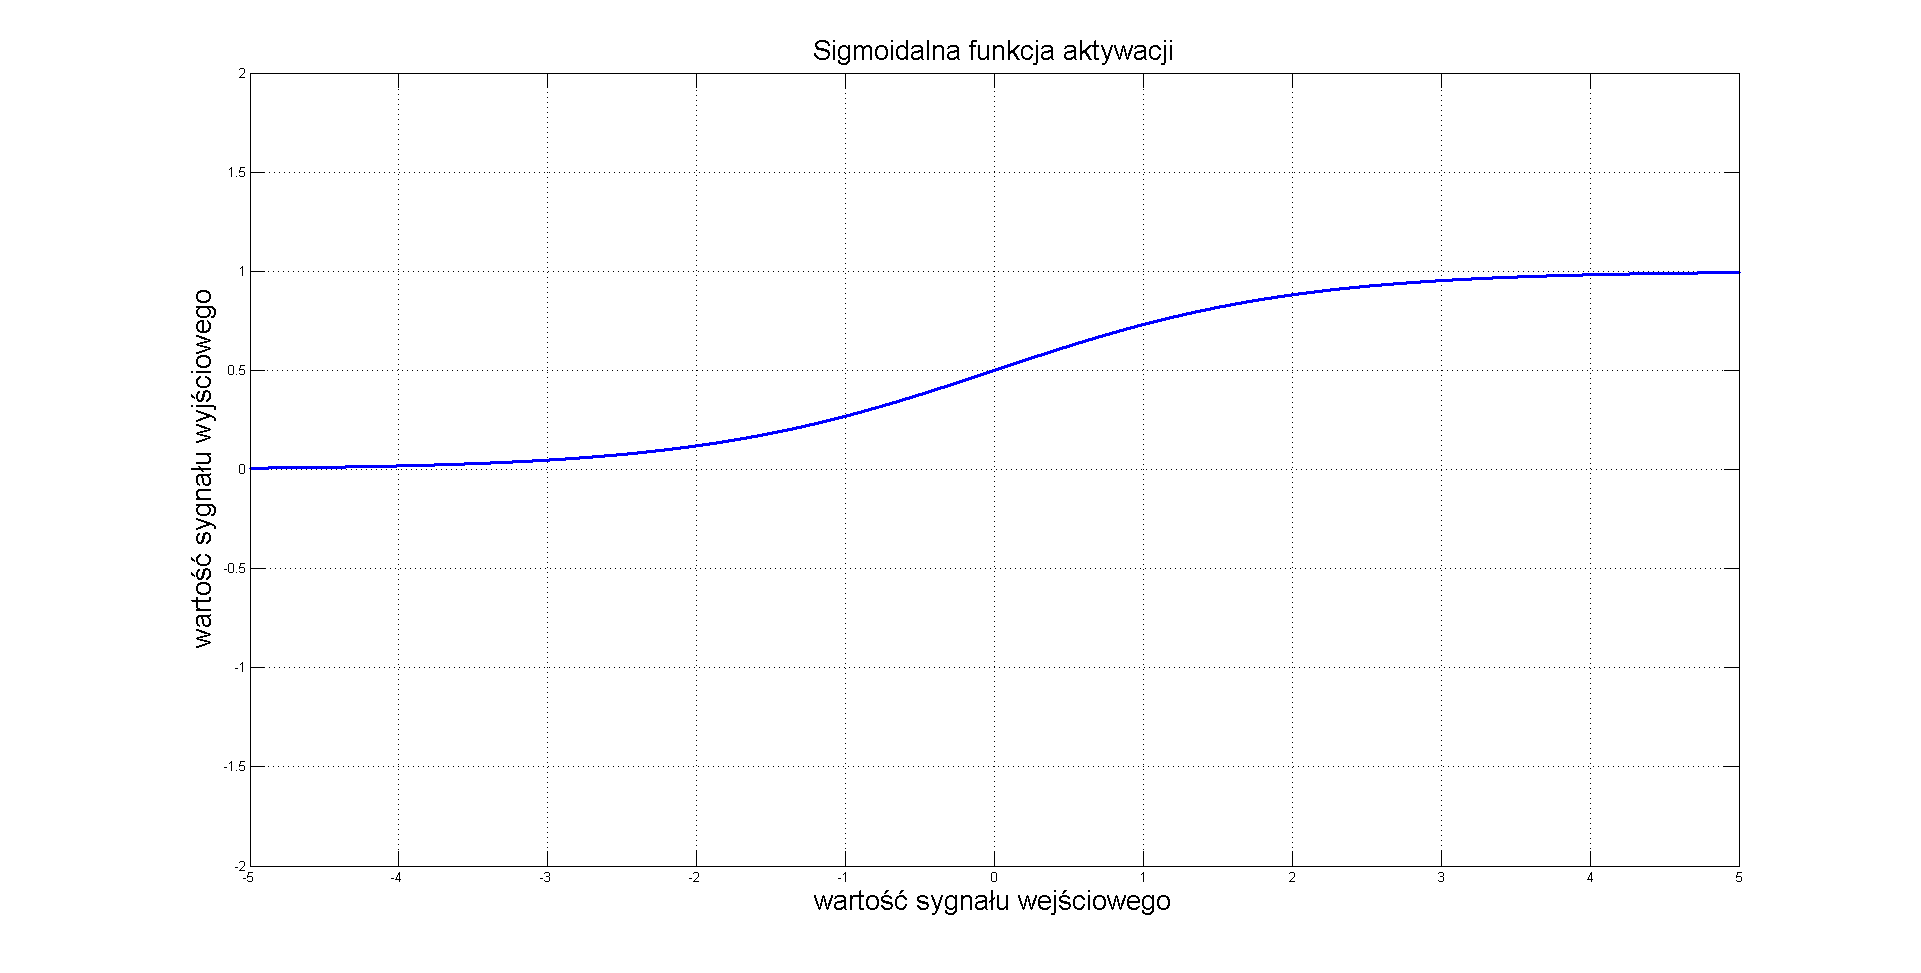
\includegraphics[width=1\linewidth]{./include/sig}
\caption{Wykres funkcji sigmoidalnej.}
\label{fig:sig}
\end{figure}

Bardzo często spotyka się również jej rozszerzoną wersję - bipolarną, przedstawioną na rysunku \ref{fig:tanh}, która opisana jest wzorem tangensa hiperbolicznego:

$$ 
f(x) = \frac{1 - e^{-x}}{1 + e^{-x}}
$$

\begin{figure}[!htbp]
\centering
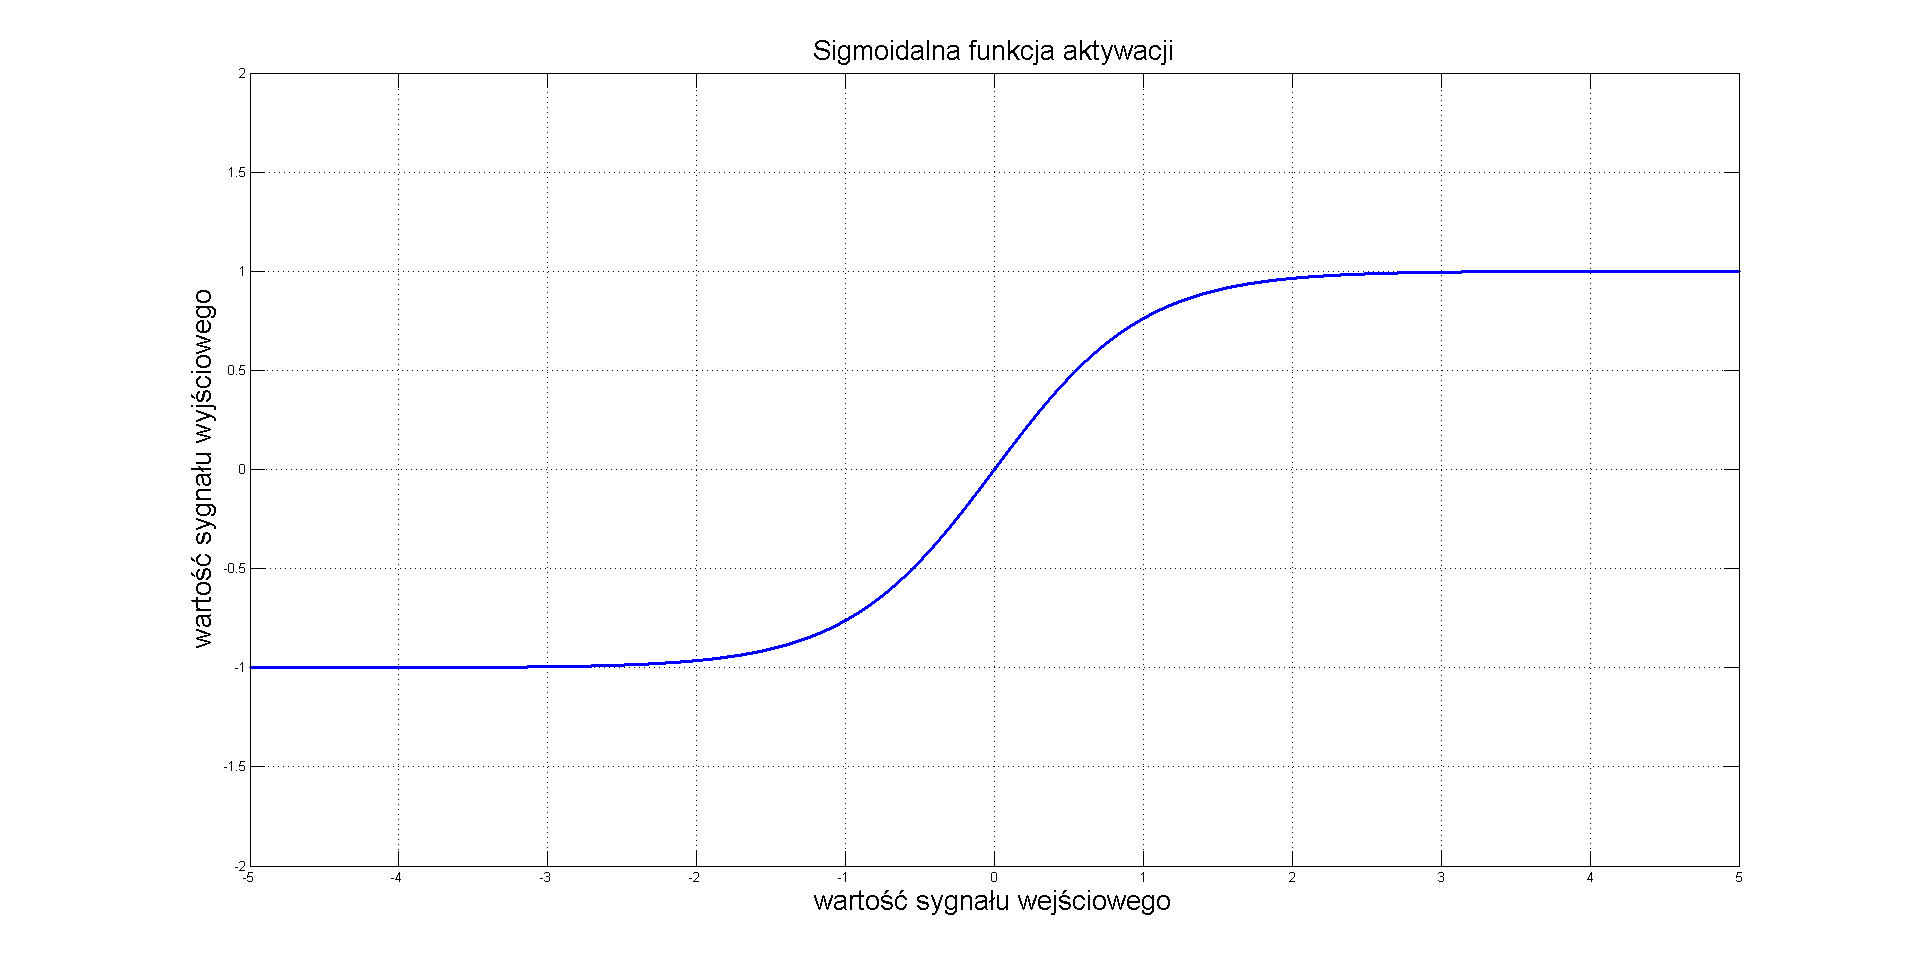
\includegraphics[width=1\linewidth]{./include/tanh}
\caption{Wykres funkcji tangensa hiperbolicznego.}
\label{fig:tanh}
\end{figure}

\section{Perceptron}
Perceptronem określa się sieć neuronową najprostszego typu, składająceją się z neuronów McCullocha-Pittsa. Ich działanie oparte jest na klasyfikacji sygnału wejściowego przez ustawienie odpowiadającego poziomu wartości wyjściowej. 
Odbywa się to poprzez równoległe przemnożenie sygnałów wejściowych przez wagi połączeń na których się znajdują. Otrzymane ilorazy są sumowane, następnie stanowią one wejście funkcji aktywacji, której wyjście reprezentuje sygnał wyjściowy całego neuronu. Powyższe operacje zostały przedstawione na rysunku \ref{fig:flow}

\begin{figure}[!htbp]
\centering
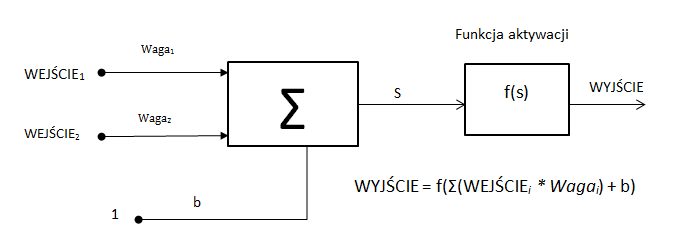
\includegraphics[width=1\linewidth]{./include/flow}
\caption{Schemat działania perceptronu.}
\label{fig:flow}
\end{figure}
 
 
Perceptrony posiadają zdolność klasyfikacji danych na charakterystyczne zbiory, które są liniowo separowalne. Własność ta pozwala tworzyć sieci, w których aktywność poszczególnego neuronu oznacza przynależność do danego zbioru. Cecha ta uniemożliwia również wytrenowanie sieci jednowarstwowej, która rozwiązywałaby problemy nieliniowe. Na przykład, sieć wykonująca operację logiczną xor, która wymaga architektury posiadającej więcej niż jedną warstwy. 
Ze względu na tą własność pojedyncza warstwa neuronów nie jest szczególnie użyteczna. Dopiero łączenie kilku warstw pozwala na rozwiązywanie złożonych problemów nieliniowych co zdecydowanie zwiększa możliwości sieci neuronowej. 

\section{Backpropagation}

Do najbardziej popularnych algorytmów uczenia sieci zaliczany jest algorytm wstecznej propagacji błędu (ang. backpropagation). Głównym założeniem tego procesu jest korekcja wag wszystkich połączeń w sieci, które wpłynęły na zwiększenie błędu wynikającego z różnicy wartości oczekiwanej i rzeczywistej. W bardzo jasny oraz szczegółowy sposób algorytm został przedstawiony w książce \cite{tade93}.

Wyróżnia się dwie najważniejsze fazy. Pierwszą z nich jest faza propagacji w przód, która podaje na wejście sieci wybrany wektor wejściowy ze zbioru danych uczących oraz odczytuje sygnał wyjściowy. Następną fazę określa się jako propagację wsteczną. Jej działanie rozpoczyna się od ostatniej warstwy sieci, do której podawana jest wartość błędu. Wykonywanie odwrotnych obliczeń wzdłuż sieci pozwala na wykrycie, które wagi wpłynęły na zwiększenie błędu, a następnie korekcję ich wartości tak, aby zminimalizować błąd. Proces ten został zobrazowany na rysunku \ref{fig:back_propagation_flow}.

\begin{figure}[!htbp]
\centering
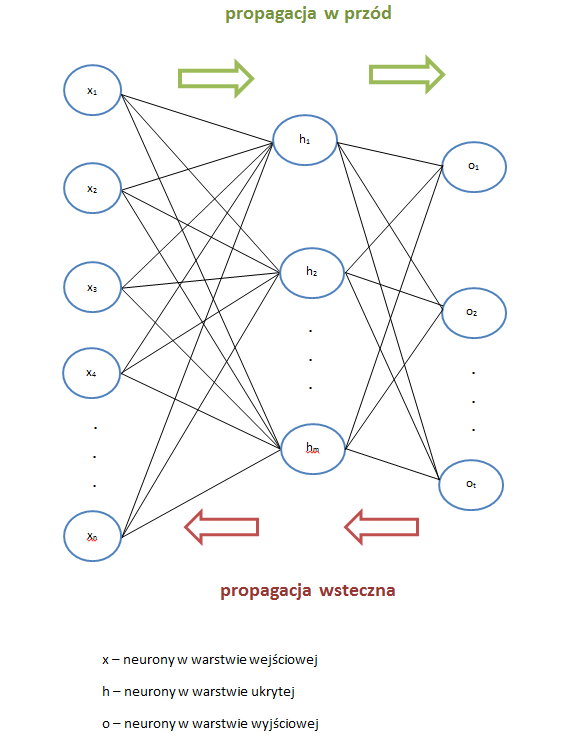
\includegraphics[width=1\linewidth]{./include/backprop_flow}
\caption{Przebieg procesu propagacji w przód oraz propagacji wstecznej.}
\label{fig:back_propagation_flow}
\end{figure}

Ze względu na istotne znaczenie tego procesu poniżej przedstawiono dokładny opis jego działania przedstawiony na pojedynczym neuronie.
Aby przystąpić do fazy nauki sieci należy odpowiednio przygotować zbiór danych uczących. Dane uczące dobierane są w ciąg o budowie opisanej wzorem \ref{eq:learning_data}.

\begin{equation}
U = <<X^{1}, z^{1}>, <X^{2}, z^{2}>,...,<X^{n}, z^{n}>>
\label{eq:learning_data}
\end{equation}

Jak łatwo zauważyć składa się on z par w postaci $<X^{j}, z^{j}>$, w których wyróżniamy wektor X z j-tym indeksem odpowiadającym krokowi w procesie uczenia oraz przypisaną do niego informacją o wartości oczekiwanej na wyjściu neuronu. Uwzględniając ówcześnie przedstawioną indeksację zbioru uczącego, regułę uczenia można opisać wzorem:

\begin{equation}
W^{j+1} = W^{j} + \eta^{j} \delta^{j} X^{j}
\label{eq:learning}
\end{equation}

We wzorze \ref{eq:learning} przyjęto:
\begin{equation}
\delta^{j} = z^{j} - y^{j}
\label{eq:delta}
\end{equation}
gdzie:
\begin{equation}
y^{j} = W^{j} * X^{j}
\label{eq:output}
\end{equation}

Reguła \ref{eq:learning} w pełni opisuje wszystkie konieczne do wykonania obliczenia. Warto jednak mieć na uwadze, iż wektor $W^{1}$ musi być określony. Bardzo często jest on inicjowany wartościami wybranymi losowo lub wartości te są przenoszone z poprzedniego procesu uczenia nawet jeśli jego zadaniem była realizacja zupełnie innej funkcji.
Bez względu na wybrany sposób inicjacji należy mieć na uwadze, aby dobrane wartości były różne $\forall_{\eta, \nu} w^{1}_{\eta} \neq w^{1}_{\nu} $. Niespełnienie tego warunku może doprowadzić do braku postępów w początkowych procesie uczenia co wpływa na jego wydłużenie, ewentualnie efekt końcowy. 

Bazując na powyższych oznaczenia można zapisać cel procesu uczenia. Celem tym jest doprowadzenie do zgodności wyjścia uczonego neurono $y^{j}$ z wartością oczekiwaną $z^{j}$, co jest jednoznaczne ze spełnieniem kryterium \ref{eq:crit}.

\begin{equation}
Q = \frac{1}{2} \sum_{j = 1}^{N} (z^{j} - y^{j})^{2}
\label{eq:crit}
\end{equation}

Dobrana funkcja $Q$ reprezentuje znaną metodę najmniejszych kwadratów.
Wzór ten można ogólnie przedstawić jako

\begin{equation}
Q = \sum_{j = 1}^{N} Q^{j}
\label{eq:common_crit}
\end{equation}

gdzie:

\begin{equation}
Q^{j} = \frac{1}{2}(z^{j} - y^{j})^{2}
\label{eq:condition_crit}
\end{equation}

Warto zauważyć, iż $Q = Q(W)$, zatem poszukiwanie minimum może odbywać się przy użyciu metody gradientowej, i-tą składową wektora $W$ można przedstawić jako:

\begin{equation}
w^{'}_i - w_{i} = \Delta w_{i} = - \eta \frac{\delta Q}{\delta w_{i}}
\label{eq:delta_member}
\end{equation}


Reasumując, proces nauczania sieci opiera się na korekcji wag poszczególnych połączeń między neuronami co powoduje minimalizowanie błędu na wyjściu sieci. Zostaje on zakończony, gdy zostanie wykonana odpowiednia liczba iteracji na zbiorze uczącym lub błąd na wyjściu będzie poniżej zadanego progu. Bardzo często spotyka się również algorytmy uczące, które zaprzestają działania gdy wprowadzane modyfikacje w następnych iteracjach są poniżej określonego progu.



